% Copyright (C) 2014-2016 by Thomas Auzinger <thomas@auzinger.name>

\documentclass[draft,final]{vutinfth} % Remove option 'final' to obtain debug information.

% Load packages to allow in- and output of non-ASCII characters.
\usepackage{lmodern}        % Use an extension of the original Computer Modern font to minimize the use of bitmapped letters.
\usepackage[T1]{fontenc}    % Determines font encoding of the output. Font packages have to be included before this line.
\usepackage[utf8]{inputenc} % Determines encoding of the input. All input files have to use UTF8 encoding.

% Extended LaTeX functionality is enables by including packages with \usepackage{...}.
\usepackage{fixltx2e}   % Provides fixes for several errors in LaTeX2e.
\usepackage{amsmath}    % Extended typesetting of mathematical expression.
\usepackage{amssymb}    % Provides a multitude of mathematical symbols.
\usepackage{mathtools}  % Further extensions of mathematical typesetting.
\usepackage{microtype}  % Small-scale typographic enhancements.
\usepackage{enumitem}   % User control over the layout of lists (itemize, enumerate, description).
\usepackage{multirow}   % Allows table elements to span several rows.
\usepackage{booktabs}   % Improves the typesettings of tables.
\usepackage{subcaption} % Allows the use of subfigures and enables their referencing.
\usepackage[ruled,linesnumbered,algochapter]{algorithm2e} % Enables the writing of pseudo code.
\usepackage[usenames,dvipsnames,table]{xcolor} % Allows the definition and use of colors. This package has to be included before tikz.
\usepackage{nag}       % Issues warnings when best practices in writing LaTeX documents are violated.
\usepackage{hyperref}  % Enables cross linking in the electronic document version. This package has to be included second to last.
\usepackage[acronym,toc]{glossaries} % Enables the generation of glossaries and lists fo acronyms. This package has to be included last.
\usepackage{xcolor}
\usepackage{listings, color}
\usepackage{pxfonts}
\usepackage{csvsimple}

% Define convenience functions to use the author name and the thesis title in the PDF document properties.
\newcommand{\authorname}{Michael Heinzl} % The author name without titles.
\newcommand{\thesistitle}{Efficient Evaluation of Well-Designed Pattern Trees with the help of In-Memory Databases} % The title of the thesis. The English version should be used, if it exists.

% Set PDF document properties
\hypersetup{
    pdfpagelayout   = TwoPageRight,           % How the document is shown in PDF viewers (optional).
    linkbordercolor = {Melon},                % The color of the borders of boxes around crosslinks (optional).
    pdfauthor       = {\authorname},          % The author's name in the document properties (optional).
    pdftitle        = {\thesistitle},         % The document's title in the document properties (optional).
    pdfsubject      = {Subject},              % The document's subject in the document properties (optional).
    pdfkeywords     = {a, list, of, keywords} % The document's keywords in the document properties (optional).
}

\setsecnumdepth{subsection} % Enumerate subsections.

\nonzeroparskip             % Create space between paragraphs (optional).
\setlength{\parindent}{0pt} % Remove paragraph identation (optional).

\makeindex      % Use an optional index.
\makeglossaries % Use an optional glossary.
%\glstocfalse   % Remove the glossaries from the table of contents.

% Set persons with 4 arguments:
%  {title before name}{name}{title after name}{gender}
%  where both titles are optional (i.e. can be given as empty brackets {}).
\setauthor{}{\authorname}{}{male}
\setadvisor{Univ.-Prof. Mag. Dr.}{Reinhard Pichler}{}{male}

% For bachelor and master theses:
\setfirstassistant{DI}{Wolfgang Fischl}{BSc}{male}

% For dissertations:
\setfirstreviewer{Pretitle}{Forename Surname}{Posttitle}{male}
\setsecondreviewer{Pretitle}{Forename Surname}{Posttitle}{male}

% For dissertations at the PhD School:
\setsecondadvisor{Pretitle}{Forename Surname}{Posttitle}{male}

% Required data.
\setaddress{Xaveriweg 4, 7000 Eisenstadt}
\setregnumber{1325545}
\setdate{19}{07}{2016} % Set date with 3 arguments: {day}{month}{year}.
\settitle{\thesistitle}{Effiziente Evaluierung von Well-Designed Pattern Trees mit Hilfe von In-Memory Datenbanken} % Sets English and German version of the title (both can be English or German).

% Select the thesis type: bachelor / master / doctor / phd-school.
% Bachelor:
\setthesis{bachelor}
%
% Master:
%\setthesis{master}
%\setmasterdegree{dipl.} % dipl. / rer.nat. / rer.soc.oec. / master
%
% Doctor:
%\setthesis{doctor}
%\setdoctordegree{rer.soc.oec.}% rer.nat. / techn. / rer.soc.oec.
%
% Doctor at the PhD School
%\setthesis{phd-school} % Deactivate non-English title pages (see below)

% For bachelor and master:
\setcurriculum{Business Informatics}{Wirtschaftsinformatik} % Sets the English and German name of the curriculum.

% For dissertations at the PhD School:
\setfirstreviewerdata{Affiliation, Country}
\setsecondreviewerdata{Affiliation, Country}

% Define convenience macros.
\newcommand{\todo}[1]{{\color{red}\textbf{TODO: {#1}}}} % Comment for the final version, to raise errors.


\definecolor{forestgreen}{RGB}{34,139,34}
\definecolor{orangered}{RGB}{239,134,64}
\definecolor{darkblue}{rgb}{0.0,0.0,0.6}
\definecolor{gray}{rgb}{0.4,0.4,0.4}

\lstdefinestyle{XML} {
    language=XML,
    extendedchars=true, 
    breaklines=true,
    breakatwhitespace=true,
    emph={},
    emphstyle=\color{red},
    basicstyle=\ttfamily,
    columns=fullflexible,
    commentstyle=\color{gray}\upshape,
    morestring=[b][\color{black}]",
    morecomment=[s]{<?}{?>},
    morecomment=[s][\color{forestgreen}]{<!--}{-->},
    keywordstyle=\color{orangered},
    stringstyle=\ttfamily\color{black}\normalfont,
    tagstyle=\color{darkblue},
	morekeywords={name,use,xmlns,version,type,minOccurs,maxOccurs,base},
	numberstyle=\small, 
 	numbersep=8pt, 
	frame = single, 
}

\lstdefinelanguage{Sparql}{
  language     = SQL,
  morekeywords = {OPTIONAL},
}


\begin{document}

\frontmatter % Switches to roman numbering.
% The structure of the thesis has to conform to
%  http://www.informatik.tuwien.ac.at/dekanat

\addtitlepage{naustrian} % German title page (not for dissertations at the PhD School).
\addtitlepage{english} % English title page.
\addstatementpage

%\begin{danksagung*}
%\todo{Ihr Text hier.}
%\end{danksagung*}
%
%\begin{acknowledgements*}
%\todo{Enter your text here.}
%\end{acknowledgements*}
%
%\begin{kurzfassung}
%\todo{Ihr Text hier.}
%\end{kurzfassung}
%
%\begin{abstract}
%\todo{Enter your text here.}
%\end{abstract}

% Select the language of the thesis, e.g., english or naustrian.
\selectlanguage{naustrian}

% Add a table of contents (toc).
\tableofcontents % Starred version, i.e., \tableofcontents*, removes the self-entry.

% Switch to arabic numbering and start the enumeration of chapters in the table of content.
\mainmatter

\chapter{Einleitung}
\section*{Motivation}
Heutzutage steht uns eine gro\ss e Menge an Daten zur Verfügung. Diese Daten werden meist in relationalen Datenbankmanagementsystemen (DBMS) verwaltet. In den 1970er wurden die ersten relationalen DBMS entwickelt und auch die Abfragesprache SQL. Zu dem Zeitpunkt der Entwicklung wurde die Annahme getroffen, dass die Daten in relationalen DBMS vollständig sind. Dies ist aber häufig nicht der Fall. In der folgenden Abbildung \ref{dbBsp} ist eine Datenbank schematisch dargestellt, welche in den nächsten Beispielen verwendet wird.

\begin{figure}[ht]
	\centering
	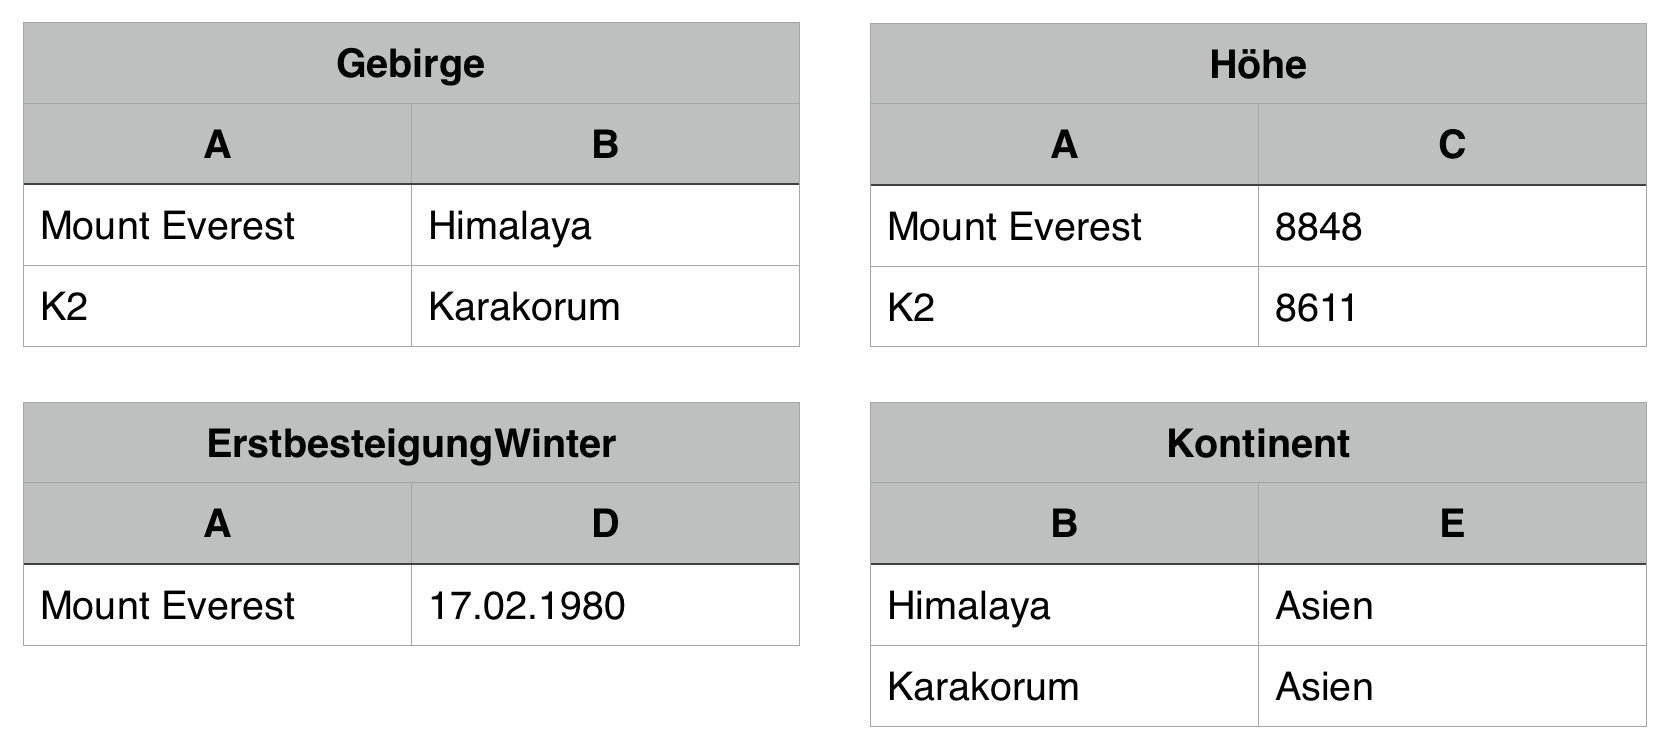
\includegraphics[width=0.9\textwidth]{DB-Beispiel}
	\caption{Datenbank Beispiel}
	\label{dbBsp}
\end{figure}

Die SQL Abfrage (Listing \ref{sqlQueryExampleDB}) liefert in diesem Fall keinen Treffer, da der Gipfel \textbf{K2} mit der Höhe von \textbf{8611} noch nie im Winter bestiegen worden ist. Diese Ergebnis kommt zustande, da die Tabelle \textit{ErstbesteigungWinter} unvollständig ist. Wenn man auf die zusätzlichen Information der Tabelle \textit{ErstbesteigungWinter} verzichtet, liefert diese Abfrage ein Ergebnis.

\begin{lstlisting}[language=SQL,caption={SELECT DB Beispiel},frame = single,label={sqlQueryExampleDB}]
SELECT Gebirge.A, Gebirge.B, ErstbesteigungWinter.D, Kontinent.E
	FROM Gebirge 
		JOIN Höhe
			ON Gebirge.A = Höhe.A
		JOIN ErstbesteigungWinter 
			ON Gebirge.A = ErstbesteigungWinter.D
		JOIN Kontinent
			ON Gebirge.A = Kontinent.E
	WHERE Höhe.C = "8611"
\end{lstlisting}



Ähnlich dazu verwendet man im Semantic Web die Abfragesprache SPARQL. SPARQL steht für \textit{SPARQL Protocol And RDF Query Language} und beruht auf dem Datenmodel RDF (Resource Description Framework). RDF ist das Standard Datenmodell des Sematic Web und ist eine Empfehlung des W3C (World Wide Web Consortium). 

Grundsätzlich ist SPARQL ein graphenbasierte Abfragesprache, welche aus drei Teilen besteht: Dem Musterabgleich, der Modifikation der Lösung und der Ausgabe. Einzeln betrachtet scheinen diese Funktionen relativ simpel, doch die Kombination macht SPARQL zu einer komplexen Sprache. In P{\'e}rez et al. 2009 \cite{PAG09} wurde dieser Themenbereich behandelt und die Klasse der \textit{well-designed SPARQL graph patterns} wurde eingeführt. Diese weisen unteranderem gute Eigenschaften für Abfrage Evaluierungen auf.

In Leteleir et al. 2013 \cite{LPPS2013} wurde eine Baumdarstellung von SPARQL Abfragen eingeführt, die sogennaten SPARQL \textit{pattern trees} und im speziellen die \textit{well-designed pattern trees} (WDPTs). Die Baumdarstellung der Abfrage spielt eine zentrale Rolle für Optimierungen. Eine besondere Bedeutung in SPARQL hat der OPTIONAL Operator. Diese Operation ermöglicht, Abfragen zu formulieren, welche das Ergebnis um gewisse Teile erweitert falls diese verfügbar sind. Dabei werden die Teilergebnisse bei denen es nicht zutrifft, nicht verworfen, sondern bleiben Teil der Lösung. In Leteleir et al. 2013 \cite{LPPS2013} wird hervorgehoben, dass mehr als 45\% der Abfragen auf dem SPARQL endpoint DBPedia den OPTIONAL Operator verwenden.

In Listing \ref{sparqlQueryExampleDB} wird gezeigt wie man durch den Einsatz des OPTIONAL Operators auch Teilergebnisse einer Abfrage erhält.

\begin{lstlisting}[float,language=Sparql,caption={SPARQL DB Beispiel},frame = single,label={sparqlQueryExampleDB}]
SELECT ?A, ?B, ?D, ?E
	WHERE { ?A Gebirge ?B . ?A Höhe "8611" . 
	OPTIONAL { ?A ErstbesteigungWinter ?D } .
	OPTIONAL { ?B Kontinent ?E }}
\end{lstlisting}

\begin{figure}[ht]
	\centering
	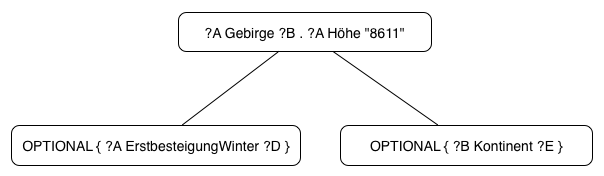
\includegraphics[width=0.9\textwidth]{SPARQL}
	\caption{SPARQL Tree}
	\label{sparqlTree}
\end{figure}

Das Ergebnis der SPARQL Abfrage (Listing \ref{sparqlQueryExampleDB}) enthält das Ergebnis der Wurzel, so wie die Teilergebnisse der OPTIONAL Knoten. (Abbildung \ref{sparqlErgebnis})

\begin{figure}[ht]
	\centering
	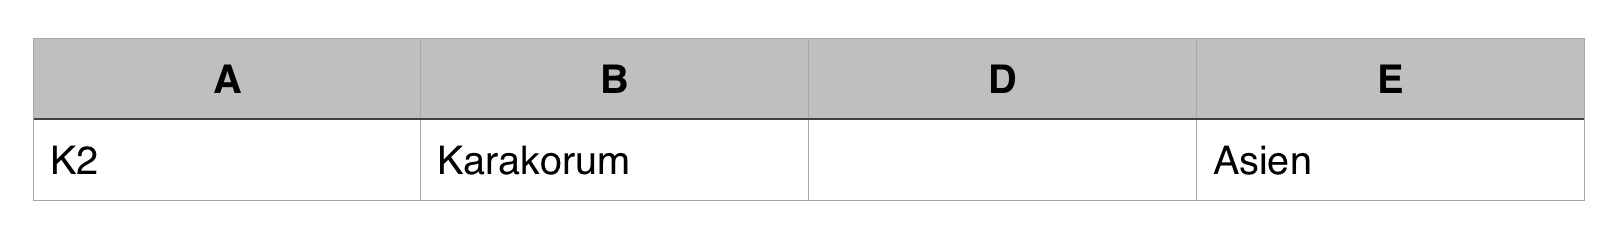
\includegraphics[width=0.9\textwidth]{sparqlErgebnis}
	\caption{SPARQL Ergebnis}
	\label{sparqlErgebnis}
\end{figure}

Conjunctive queries (Select-From-Where Abfragen) sind die Grundlage der heutigen DBMS. Diese Art von Abfragen haben ein Problem mit unvollständigen bzw. semistrukturierten Daten. Wenn eine Abfrage nicht exakt mit den Daten übereinstimmt, kann keine Antwort ermittelt werden. Hier kommt wiederum der OPTIONAL Operator zur Anwendung. Dieser entspricht in der relationalen Algebra grundsätzlich dem LEFT OUTER JOIN (Barcelo et al. 2015 \cite{DBLP:conf/pods/BarceloPS15}). 

Die Arbeit beschäftigt sich im Weiteren mit der effizienten Evaluierung der WDPTs. Diese Evaluierung wird mit Hilfe eines DBMS und des LEFT OUTER JOIN realisiert. Um eine möglichst effiziente Auswertung zu ermöglichen wird eine In-Memory Datenbank verwendet. In-Memory Datenbanken haben den Vorteil, dass die Daten nur im Arbeitsspeicher gehalten werden und somit schneller Ergebnisse liefern können. 

\section*{Ziel}
Die derzeitige Implementierung des Algorithmus \cite{DBLP:conf/www/AhmetajFPSS15} basiert auf einem einfachen iterativen Vorgehen. Das Ziel ist die Implementierung eines Algorithmus, welcher unter Zuhilfenahme einer In-Memory Datenbank die Leistung verbessert und somit die Durchlaufzeit verringert. Bei diesen Tests kommen verschiedene In-Memory Datenbanken zum Einsatz, um für diesen speziellen Anwendungsfall eine geeignete Implementierung auszuwählen.

\section*{Aufbau der Arbeit}
Die Arbeit ist folgenderma{\ss}en aufgebaut. Zu Beginn in Kapitel \ref{istZustand} wird die derzeitige Implementierung beschrieben und analysiert. Im speziellen wird die Leistung des derzeitigen Algorithmus als Orientierungswert für den späteren Vergleich herangezogen. Des Weiteren wird die Datenstruktur der Eingabedaten erläutert, diese Daten dienen als Eingabe für die derzeitige und zukünftige Implementierung.

Das Kapitel \ref{inMemoryDatenbanken} beschäftigt sich mit Konzepten und Anforderungen im Bereich In-Memory Datenbanken. 

Danach wird im Kapitel \ref{umsetzung} die neue Implementierung unter der Verwendung von einer In-Memory Datenbank erläutert. Abschlie{\ss}end wird der neue Algorithmus mit dem bisherigen Algorithmus verglichen.

\chapter{Basisdefinitionen}
\paragraph{RDF}
Resource Description Framework (RDF) ist ein Datenmodell für den Datenaustausch im Web. Die Grundstruktur begünstigt das Zusammenführen von Daten, auch wenn sich die zugrundeliegenden Schemen unterscheiden. Ein weiterer Vorteil liegt darin, dass einfach Änderungen am Schema vorgenommen werden können ohne, dass sich der Benutzer anpassen muss. RDF baut auf der Struktur von URIs auf. URIs werden verwendet, um ein Verknüpfung und deren Enden zu identifizieren. Diese Verknüpfung ergibt ein Tripel.
$U$ ist eine abzählbar unendliche Menge aus URIs. Ein RDF Tripel $t$ ist jedes Tupel $t \in U \times U \times U$. Ein RDF Graph $G$ ist jene Menge $G \subseteq U \times U \times U$ aus Tripeln. Leere Knoten sind nicht zulässig. \\ \cite{rdfSite}  

\paragraph{SPARQL}
SPARQL Protocol And RDF Query Language (SPARQL) ist eine graphenbasierte Abfragesprache für RDF.  Sei $V$ eine unendliche Menge an Variablen. $U \cap V = \emptyset$ Variablen werden mit einem führenden Fragezeichen markiert z.B. ?x. Ein SPARQL Tripel $t$ ist ein Tupel in $(U \cup V) \times (U \cup V) \times (U \cup V)$.  

\begin{lstlisting}[language=Sparql,caption={SPARQL Beispiel},frame = single,label={sparqlQueryExample}]
SELECT ?A, ?B, ?D
	WHERE { ?A Gebirge ?B . ?A Höhe "8611" . 
	OPTIONAL { ?A ErstbesteigungWinter ?D }}
\end{lstlisting}

Das Listing \ref{sparqlQueryExample} zeigt ein Beispiel einer SPARQL Abfrage. Der SELECT Teil wählt die Variablen für das Ergebnis aus. Im WHERE Teil wird das Anfragemuster dargestellt, dieses verwendet die Tripel Syntax. Der Punkt repräsentiert eine AND Verknüpfung. Der OPTIONAL Operator fügt die Teilergebnisse nur hinzu, wenn diese vorhanden sind.

\cite{SPARQL}


\paragraph{WDPT}
Ein Graph welcher nur die Operatoren AND und OPT enthält ist in OPT Normalform, wenn die OPTIONAL Operatoren nicht im Geltungsbereich eines AND Operator vorkommt. Es wurde gezeigt, dass jeder \textit{well-designed graph pattern} in OPT Normalform umgewandelt werden kann. Ein \textit{pattern tree} (PT) $X$ ist ein Paar aus $(T,P)$ wobei $T = (V,E,r)$ ein ungeordneter Baum ist und $P = \{P_n \, | \, n \in V\}$ ist die Beschriftung der Knoten in $V$ ist. Ein \textit{well-designed pattern tree} ist ein \textit{pattern tree }$X = (T,P)$, welcher für jede Variable $?x \in vars(X)$, die Knoten $\{n \in V(X)\, | \, ?x \in vars(n)\}$ einen verbunden Subgraphen beinhalten. 

\cite{DBLP:conf/www/AhmetajFPSS15}

\chapter{Ist-Zustand} \label{istZustand}
\section{Datenstruktur} \label{dataStruk}
Der Ausgangspunkt des Algorithmus ist eine XML-Datei, diese repräsentiert die Auswertung  mehrerer Knoten in einem Well-Designed Pattern Tree (WDPT). Das Schema der XML-Datei ist unter Listing \ref{lst:xsd} definiert und wird im weiteren genauer erläutert.

Die XML-Datei enthält ein Hauptelement \textit{ptresult}. Dieses wiederum enthält eine Sequenz von Elementen \textit{ovar}, welche die Variablen der Projektion des WDPT abbilden \cite{OptMat}. Des Weiteren enthält \textit{ptresult} den Wurzelknoten des Well-Designed Pattern Tree. Dieser wird durch ein \textit{node} Element dargestellt.

Der Wurzelknoten des Baums ist die Basis des WDPT. Alle weiteren Kindknoten stellen die Auswertung einer OPTIONAL-Klausel da. Die OPTIONAL-Klauseln können auch geschachtelt verwendet werden, infolgedessen ergibt sich eine Baumstruktur. Diese Knoten sind ebenfalls durch die Elemente \textit{node} abgebildet. Ein \textit{node} Element besteht aus genau einem \textit{variables} Element, beliebig vielen \textit{mapping} Elementen und danach beliebig vielen \textit{node} Elementen. Diese \textit{node} Elemente stellen die Kindknoten dar.

Das \textit{variables} Element enthält mehrere \textit{nodeVar} Elemente. Diese repräsentieren die Variablen, welche innerhalb der zugehörigen OPTIONAL-Klausel des Knotens verwendet werden.

Nun zum eigentlichen Kernstück der XML-Datei. Das \textit{mapping} Element ist eine konkrete Belegung von Variablen der SPARQL-Abfrage. Diese enthalten die eigentlichen Daten. Somit enthält das \textit{var} Element die konkreten Ausprägungen der SPARQL-Variablen, der Name dieser Variable ist dazu in dem Attribut \textit{name} des \textit{var} Elements hinterlegt.\\

\pagebreak

\lstinputlisting[style=XML,caption={XML Schema der Eingabedatei},label={lst:xsd}]{input.xsd}
Weiters ist unter Listing \ref{lst:xml} eine Beispiel XML-Datei angegeben, welche später als Referenz dient.
\lstinputlisting[style=XML,caption={Beispiel XML Eingabedatei},label={lst:xml}]{test.xml}

Der Well-Designed Pattern Tree (WDPT) der XML-Datei (Listing \ref{lst:xml}) ist in Abbildung \ref{wdptBsp} dargestellt.
\begin{figure}[ht]
	\centering
	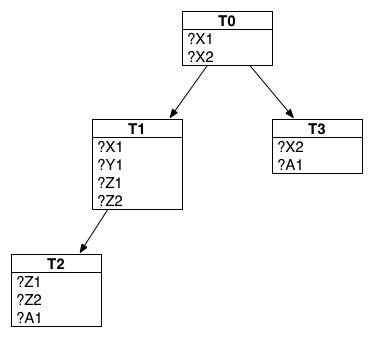
\includegraphics[width=0.5\textwidth]{WDPT}
	\caption{WDPT der beschriebene XML-Datei (Listing \ref{lst:xml})}
	\label{wdptBsp}
\end{figure}

\section{Implementierung} \label{istImp}

Die aktuelle Implementierung ohne In-Memory Datenbank besteht aus mehreren Phasen:

\paragraph{Einlesen}
Die erste Phase besteht darin, eine oben beschriebene XML-Datei einzulesen und die XML-Strukturen in folgende Java Objekte zu konvertieren.

Die Klasse \textit{EvalPT} spiegelt das Hauptelement \textit{ptresult} der XML-Datei wieder. Die Klasse enthält den Wurzelknoten, so wie die Variablen der \textit{ovar} Elemente. Die \textit{node} Elemente werden in in der Klasse \textit{EvalTreeNode} abgebildet. Die Einträge aus dem \textit{variables} Element werden als \textit{Set} in dieser Klasse gespeichert. Zusätzlich enthält die Klasse auch eine Liste von Kindknoten des Typs \textit{EvalTreeNode}. Der Gro\ss teil der zu verarbeitenden Daten besteht aus den \textit{mapping} Elementen, dies werden in dem entsprechenden \textit{EvalTreeNode} Objekt in einem \textit{Set} gespeichert. Die \textit{mapping} Elemente werden in Java als \textit{Map} abgebildet. Die Variablennamen bilden die Schlüssel und die konkreten Ausprägungen der SPARQL-Variablen bilden die Werte der \textit{Map}. Diese \textit{Map} Objekte werden im Folgenden als Mapping bezeichnet. In Abbildung \ref{klassendiagramm} sind die Klassen als Klassendiagramm dargestellt. 

\begin{figure}[ht]
	\centering
	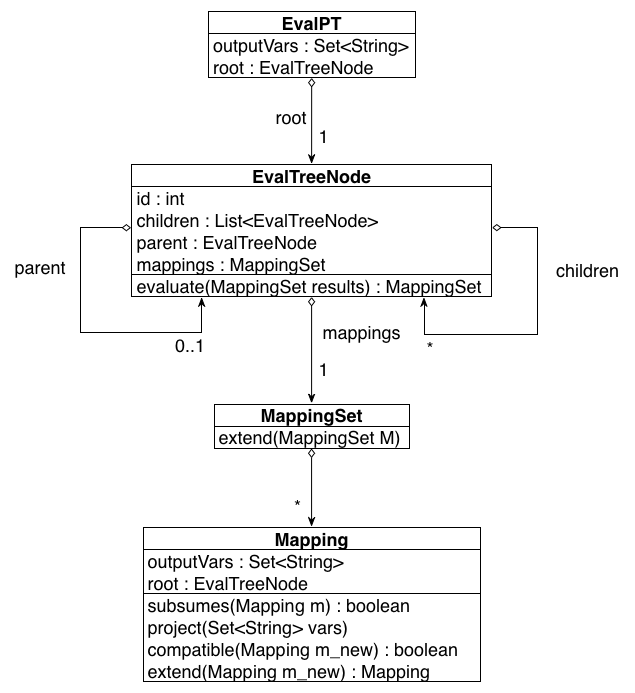
\includegraphics[width=0.9\textwidth]{Klassendiagramm}
	\caption{Klassendiagramm}
	\label{klassendiagramm}
\end{figure}

\paragraph{Vereinigung}
Die zweite Phase des Algorithmus beschäftigt sich mit der eigentlichen Vereinigung des Wurzelknotens und aller Kindknoten. Der Vorgang beginnt bei dem Wurzelknoten, es wird hierbei ein neues \textit{Set} aus Mapping Objekten angelegt, dieses wird im Folgenden als \textit{results} bezeichnet. Als Initialwerte wird \textit{results} mit den Mappings des Wurzelknoten befüllt. Nun werden diese Mappings um passende Mappings aller Kindknoten erweitert. Für jeden Kindknoten werden folgende Schritte durchgeführt:

\paragraph{Kompatibilität}
Für jedes Mapping in \textit{results} wird für jedes Mapping im Kindknoten überprüft, ob dieses Mappings mit einander kompatibel sind. Zwei Mappings sind mit einander kompatibel, wenn bei dem paarweisen Vergleich alle übereinstimmenden Variablen auch den selben Wert aufweisen. Der Pseudo-Code für die Kompatibilität zweier Mappings ist in Algorithmus \ref{alg:komp} zu finden. \\ In Listing \ref{bspKompMap} sind zwei Beispiele zu finden. \textit{m1} und \textit{m2} sind kompatible Mappings, da die gemeinsamen Variablen (\textit{?X}, \textit{?Y}) auch den gleichen Wert aufweisen. Hingegen sind \textit{m3} und \textit{m4} nicht kompatibel, da die Variable \textit{?Z} unterschiedliche Werte aufweist.

\begin{algorithm}
\SetKwData{Left}{left}\SetKwData{This}{this}\SetKwData{Up}{up}
\SetKwFunction{Union}{Union}\SetKwFunction{FindCompress}{FindCompress}
\SetKwInOut{Input}{input}\SetKwInOut{Output}{output}
\Input{Mapping $m1$ und Mapping $m2$}
\Output{true wenn $m1$ mit $m2$ kompatibel sind, sonst false}
\BlankLine
$keys1\leftarrow$ Menge der Schlüssel von $m1$\;
$keys2\leftarrow$ Menge der Schlüssel von $m2$\;
$interKeys\leftarrow m1\cap m2$\;
\ForEach{Schlüssel k aus $interKeys$}{
  $v1\leftarrow m1[k]$\;
  $v2\leftarrow m2[k]$\;
  \If{$v1\neq v2$}{
    \Return false\;
  }
}
\Return true\;
\caption{Kompatibilität von zwei Mappings}\label{alg:komp}
\end{algorithm}

\begin{lstlisting}[float,caption={Beispiele für Kompatibilität von zwei Mappings},frame=single,label={bspKompMap}]
// Kompatibel
m1 = {
	(?X, "x"), (?Y, "y"), (?Z, "z")	
}

m2 = {
	(?X, "x"), (?Y, "y"), (?A, "a")	
}

// Nicht Kompatibel
m3 = {
	(?X, "x"), (?Y, "y"), (?Z, "z")	
}

m4 = {
	(?X, "x"), (?Y, "y"), (?Z, "a")	
}
\end{lstlisting}

Wenn das Mapping aus \textit{results} mit dem Mapping aus dem Kindknoten kompatibel ist, wir das Mapping aus \textit{results} um die neuen Variablen und deren Werten erweitert (siehe Algorithmus \ref{alg:erw}). Nach dem jedes Mapping aus \textit{results} mit allen Mappings des Kindknoten abgeglichen wurde, ist dieser Kindknoten fertig abgearbeitet. Danach durchlaufen die Kindknoten des jetzigen Knoten die selbe Prozedur. Bei jedem Kindknoten wird \textit{results} um einige Werte erweitert. Diese Phase ist beendet, wenn alle Knoten im Baum abgearbeitet sind. Nun enthält \textit{results} alle erweiterten Mappings.

\begin{algorithm}
\SetKwInOut{Input}{input}
\Input{Set $results$ aus Mappings, Set $M$ aus Mappings}
\BlankLine
MappingSet $toAdd \leftarrow$ leeres Set\;
\ForEach{Mapping $m1$ aus $results$}{
  $added\leftarrow false$\;
  \ForEach{Mapping $m2$ aus $M$}{
    \If{$m1$ kompatibel mit $m2$}{
      Mapping $extendedMapping \leftarrow$ Erweitere $m1$ mit $m2$\;
	  Füge $extendedMapping$ zu $toAdd$ hinzu\;
	  $added\leftarrow true$\;
    }
  }
  \If{$added$}{
    Entferne $m1$ aus $results$ da $m1$ mindestens einmal erweitert wurde und am Ende hinzugefügt wird\;
  }
}
Füge alle Mappings aus $toAdd$ zu $results$ hinzu\;
\caption{Erweiterung der MappingSets}\label{alg:erw}
\end{algorithm}

\begin{lstlisting}[float,caption={Beispiele für Erweiterung der MappingSets},frame=single,label={bspKompMap}]
MappingSet results = { 
	{ (?X, "x1"), (?Y, "y1") }, 
	{ (?X, "x2"), (?Y, "y2") } 
}

MappingSet M = { 
	{ (?X, "x1"), (?A, "b1") }, 
	{ (?X, "x2"), (?B, "b2") },
	{ (?X, "x2"), (?C, "c1") }
}

//Erweiterung von results mit M
results = { 
	{ (?X, "x1"), (?Y, "y1"), (?A, "b1") }, 
	{ (?X, "x2"), (?Y, "y2"), (?B, "b2") },
	{ (?X, "x2"), (?Y, "y2"), (?C, "c1") }
}
\end{lstlisting}

In der dritten Phase findet die Projektion der Daten statt. Hierbei wird über alle Mappings iteriert und es werden alle Variablen entfernt, welche nicht in der Projektion (\textit{ovar} Elemente) enthalten sind. 

\paragraph{Maximierung} \label{maxMapPar}
Die vierte und letzte Phase beschäftigt sich mit der Maximierung der Mappings (\cite{DBLP:conf/www/AhmetajFPSS15} unter CERTAIN ANSWER SEMANTICS) aus \textit{results}. Alle Elemente aus \textit{results} werden in eine neue Menge \textit{maxResults} überführt. Zu Beginn ist die Menge \textit{maxResults} leer. Die Elemente aus \textit{results} werden einzeln in \textit{maxResults} eingefügt. Um ein Element zur Menge hinzuzufügen wird Algorithmus \ref{alg:max} angewandt.

Der Algorithmus verwendet die Funktion \textit{subsums}. Diese erhält zwei Eingabeparameter Mapping \textit{m1} und Mapping \textit{m2}. Sie überprüft wie folgt, ob \textit{m1} \textit{m2} subsumiert. Ist die Anzahl der Elemente von \textit{m1} kleiner als die von \textit{m2}, subsumiert \textit{m1} nicht \textit{m2}. Ist das nicht der Fall, wird die Schlüssel der Mappings verglichen. Wenn \textit{keys1} die Schlüssel von \textit{m1} sind und \textit{keys2} die Schlüssel von \textit{m2} sind, dann subsumiert \textit{m1} \textit{m2} nicht, wenn \textit{keys1} nicht alle Schlüssel aus \textit{keys2} beinhaltet. Ist das nicht der Fall wird über alle Schlüssel aus \textit{keys2} iteriert. Wenn \textit{k} ein Schlüssel aus \textit{keys2} ist, müssen die Werte der Mappings für \textit{k} für alle Elemente aus \textit{keys2} gleich sein. Trifft das zu, dann subsumiert \textit{m1} \textit{m2}. Unter Listing \ref{subsumBsp} ist ein Beispiel zu finden. 

Zu Beginn des eigentlichen Algorithmus wird überprüft ob das einzufügende Element \textit{newM} schon in dem Set \textit{maxResults} vorhanden ist, wenn das der Fall ist, wird das Element nicht erneut eingefügt und der Algorithmus ist beendet. Danach wird über das Set \textit{maxResults} iteriert. Wenn \textit{oldM} ein Mapping aus dem Set \textit{maxResults} ist, wird überprüft ob \textit{oldM} \textit{newM} subsumiert. Ist das der Fall, wird \textit{newM} nicht in das Set eingefügt und der Algorithmus ist beendet. Wenn \textit{newM} \textit{oldM} subsumiert wird \textit{oldM} aus \textit{maxResults} entfernt. Subsumiert keines der Mappings aus \textit{maxResults} \textit{newM}, wird \textit{newM} zu \textit{maxResults} hinzugefügt.

\begin{lstlisting}[float,caption={Beispiel für Subsumierung},frame=single,label={subsumBsp}]
Mapping m1 = { ("?X","x"), ("?Y","y"), ("?Z","z"), ("?A","a") }

Mapping m2 = { ("?X","x"), ("?Y","y"), ("?B","b") }
//m1 subsumiert NICHT m2

Mapping m3 = { ("?X","x"), ("?Y","y"), ("?Z","b") }
//m1 subsumiert NICHT m3

Mapping m4 = { ("?X","x"), ("?Y","y"), ("?Z","z") }
//m1 subsumiert m4
\end{lstlisting}

\begin{algorithm}
\SetKwInOut{Input}{input}
\SetKwFunction{Subsums}{subsums}
\Input{Set $maxResults$, Mapping $newM$}
\BlankLine
$isSubsumed\leftarrow false$\;
\If{$maxResults$ enthält $newM$}{return\;}
\ForEach{Mapping $oldM$ aus $maxResults$}{
  \If{\Subsums{oldM, newM}}{
    $isSubsumed\leftarrow true$\;
    break\;
  }
  \If{\Subsums{newM, oldM}}{
    Entferne $oldM$ aus $maxResults$\;
  }
}
\If{!isSubsumed}{
  Füge $newM$ in $maxResults$ ein\;
}
\SetKwProg{Fn}{function}{}{end}
\BlankLine
\Fn{Boolean subsums(Mapping m1, Mapping m2)}{
  \eIf{Anzahl der Elemente von m1 $\geq$ Anzahl der Elemente von m2}{
    $keys1\leftarrow$ Schlüssel von $m1$\;
    $keys2\leftarrow$ Schlüssel von $m2$\;
    \eIf{$keys1$ beinhaltet alle Elemente aus $keys2$}{
      \ForEach{Schlüssel $k$ aus $keys2$}{
        $v1\leftarrow m1[k]$\;
        $v2\leftarrow m2[k]$\;
        \If{$v1\neq v2$ AND $v2\neq null$}{
          \Return false\;
        }
      }
    }{
      \Return false\;
    }
  }{
    \Return false\;
  }
  \Return true\;
}
\caption{Hinzufügen zu MaxSet}\label{alg:max}
\end{algorithm}

Dieser prozedurale Algorithmus ist in \cite{OptMat} unter Top-Down Evaluation zu finden.

\pagebreak

\section{Benchmarking} \label{benchmarking}

Die Zeitmessung des aktuellen Systems beruht auf mehreren Etappen, in welchen über die Java Funktion \textit{System.nanoTime()} die vergangene Zeit seit der letzen Etappe gemessen wird. Folgende Etappen wurden gemessen:
\begin{enumerate}
	\item Read - Die Zeit für das Einlesen der Datei
	\item Evaluation - Die Auswertung der Daten ohne Maximierung des Ergebnisses
	\item MaxSet - Die Maximierung des Ergebnisses
\end{enumerate}

Es wurden jeweils drei Durchläufe erfasst. Am Ende wurden die Ergebnisse der Etappen aufsummiert. Weiters wurden die durchschnittlichen Zeiten der Durchläufe pro Etappe errechnet.

Diese Dateien wurden zum Test herangezogen:
\begin{itemize}
	\item lubm-ex-20-15.sparql.xml
	\begin{itemize}
		\item Dateigrö{\ss}e: 2,44 MB
		\item Zeilenanzahl: 40.827
		\item Auswertungsergebnis: 
		\begin{itemize}
			\item Zusammenfassung in Listing \ref{lst:bi15}
			\item Rohdaten in Listing \ref{lst:bi15raw}
		\end{itemize}
	\end{itemize}
	\item lubm-ex-20-17.sparql.xml
	\begin{itemize}
		\item Dateigrö{\ss}e: 24,95 MB
		\item Zeilenanzahl: 378.450
		\item Auswertungsergebnis: 
		\begin{itemize}
			\item Zusammenfassung in Listing \ref{lst:bi17}
			\item Rohdaten in Listing \ref{lst:bi17raw}
		\end{itemize}
	\end{itemize}
\end{itemize}

Es fällt auf, dass die Phase Evaluierung den grö\ss ten Optimierungsbedarf aufweist. Bei der kleineren Datei lubm-ex-20-15.sparql.xml benötigt die Evaluierung nur knapp länger als die Maximierung. Bei der grö\ss eren Datei lubm-ex-20-17.sparql.xml ist die Maximierung zu vernachlässigen, da diese Phase nur ca. 0,04\% der Gesamtdauer in Anspruch nimmt. Weiters fällt auf, dass bei steigender Dateigrö\ss e die Phase Einlesen nicht so stark zunimmt wie die Phase Evaluierung.

Aus \textit{LUBM: A benchmark for OWL knowledge base systems} \cite{Guo2005158} und \textit{Towards Reconciling {SPARQL} and Certain Answers --- Extended Version.} \cite{ahmetaj2015wwwext} wurden die oben angeführten Dateien generiert.
Alle Zeitangaben sind in Sekunden angegeben.

\begin{lstlisting}[basicstyle=\tiny,caption={Benchmark ITERATIVE, Datei: lubm-ex-20-15.sparql.xml},label={lst:bi15}]
+=======================================================================+
| Einlesen        | Evaluierung     | Maximierung     | Summe           | 
+=======================================================================+
| 0.185869        | 7.136303        | 7.037891        | 14.360063       |
+=======================================================================+
\end{lstlisting}

\begin{lstlisting}[basicstyle=\tiny,caption={Benchmark ITERATIVE, Datei: lubm-ex-20-17.sparql.xml},label={lst:bi17}]
+=======================================================================+
| Einlesen        | Evaluierung     | Maximierung     | Summe           | 
+=======================================================================+
| 1.022490        | 484.785088      | 0.190920        | 485.998499      |
+=======================================================================+
\end{lstlisting}

\chapter{In-Memory Datenbanken} \label{inMemoryDatenbanken}
Die folgenden Abschnitte befassen sich mit neuen Anforderungen und Konzepten im Bereich In-Memory Datenbanken. Verwendete Literatur: \cite{BookInMem}
\section{Neue Anforderungen an Datenbanksysteme}
Wenn man heutzutage ein von Grund auf neues Datenbanksystem entwickeln würde, hätte dieses andere Anforderungen als konventionelle Datenbanksysteme. Moderne Unternehmen arbeiten täglich mit einer Fülle von Daten, was vor ein paar Jahren noch undenkbar war. Fertigungsunternehmen sind ein Beispiel, für solche datenlastige Betriebe. Während des Fertigungsprozesses werden enorme Mengen an Daten produziert. Diese müssen oft in Echtzeit verarbeitet werden und liefern Grundlagen für weitere Entscheidungsprozesse. Dies ist nur ein Beispiel der steigenden Bedürfnisse moderner Datenbanksysteme. 

Es gibt zwei wesentliche Anforderungen für moderne Datenbanksysteme. Daten aus unterschiedlichen Eingabequellen müssen in einem Datenbanksystem aufgenommen werden und diese Daten müssen in Echtzeit verarbeitet werden, um abgestimmte Entscheidungen treffen zu können. Die weiteren Abschnitte beschreiben verschiedene Einsatzgebiete, in denen diese Anforderungen zu tragen kommen.

\subsection*{Ereignisdaten}
Ereignisdaten sind der Kern zukünftiger Produktionsanlagen, diese sind wie folgt charakterisiert. Die Datenmenge eines einzelnen Elements ist sehr klein, nur ein paar Bytes oder Kilobytes gro\ss . Im Gegenzug ist die Anzahl der Ereignisse für eine gewisse Einheit im Verhältnis enorm hoch. 

In der Produktion von alltäglichen Produkten kommt eine Vielzahl von Sensoren zum Einsatz. Besonders in den Bereichen heikler Produkte müssen alle Schritte der Produktion und Auslieferung dokumentiert werden. Um Produkte während dieser Prozesse genau beobachten zu können, werden RFID (Radio Frequency Identification) Tags oder zweidimensionale Strichcodes eingesetzt. Bei jedem Schritt der Produktion bzw. der Auslieferung kommen Sensoren zum Einsatz, um den Weg des Produktes zu identifizieren. 

BigPoint ist ein Spieleentwickler mit dem Sitz in Deutschland. In der Spieleindustrie sind Ereignisdaten von zentraler Bedeutung. BigPoint verwendet diese Daten, um in Echtzeit den Spielern in schwierigen Situationen zahlungspflichtige Hilfen anzubieten. Diese Spiele produzieren 10.000 Ereignisse pro Sekunde. Herkömmliche Datenbanken sind für diesen Anwendungszweck nur begrenzt einsetzbar. Flexible und auf den Anwendungsfall zugeschnittene Abfragen von Entwicklern können nicht interaktiv beantwortet werden. In-Memory Datenbanken werden eingesetzt, um in kürzester Zeit Entscheidungen über den Einsatz von zahlungspflichtigen Hilfen zu treffen. Es werden verschiedene Gruppen von Spielern analysiert und es wird entschieden ob alle Spieler diese Angebote bekommen.

\subsection*{Strukturierte und unstrukturierte Daten}
Man muss zwischen strukturierten und unstrukturierten Daten unterscheiden. Strukturierte Daten weisen ein Schema auf, auf Basis dessen man die Daten analysieren kann. Daten welche in relationalen Datenbanken gespeichert werden, sind zum Beispiel strukturierte Daten. Im Gegensatz dazu weisen unstrukturierte Daten kein Schema auf, somit kann nicht so einfach eine Analyse der Daten vorgenommen werden, z.B.: Bilder, Videos, freie Texte, etc. Im Laufe der Zeit sind in vielen Unternehmen eine gro\ss e Menge von unstrukturierten Daten wie Berichte, Tabellen oder Textdokumente angefallen. In diesen unstrukturierten Daten verbirgt sich eine Menge an Informationen. Es besteht eine enorme Nachfrage, in diesen Dokumenten schnell und flexibel nach Informationen zu suchen.

In Spitälern sammeln sich gro\ss e Mengen von strukturierten und unstrukturierten Patientendaten an. In-Memory Datenbanken ermöglichen die Kombination von strukturierten und unstrukturierten Daten, so wie die Einbindung von externen Daten z.B. klinischen Studien oder Nebenwirkungen. Somit können Ärzte in Echtzeit, die benötigten Daten interaktiv kombinieren und schneller Diagnosen stellen. Dieser Prozess verringert die manuelle und zeitaufwendige Arbeit der Ärzte enorm.

Auch bei Wartungsarbeiten von Flugzeugen werden In-Memory Datenbanken eingesetzt. Bei der Bearbeitung von Wartungsaufträgen fallen strukturierte wie auch unstrukturierte Daten an. Mit Hilfe der In-Memory Technologie können Korrelationen zwischen Schwachstellen erkannt werden und dies wiederum kann das Risiko eines Fehlers verringern.

In Spitälern wie auch in der Flugzeug Industrie spielt die Zeit und somit die Dauer einer Datenbankabfrage, vor allem in Notfällen, eine wichtige Rolle. Durch In-Memory Datenbanken können auch zeitkritische Abfragen oder Operationen auf mobilen Endgeräten durchgeführt werden.
\section{Konzepte}
Die folgenden Abschnitte beschäftigen sich mit den verwendeten Konzepten in einer In-Memory Datenbank, am Beispiel der SanssouciDB. Die SanssouciDB ist ein modellhaftes Datenbanksystem, welches auf Prototypen des Hasso-Plattner-Institut und auf eine existierende SAP Datenbank aufbaut. SanssouciDB ist eine SQL Datenbank mit ähnlichen Komponenten wie eine gewöhnliche Datenbank.

\subsection{Verwendung des Hauptspeichers}
Der gro\ss e Unterschied zwischen In-Memory Datenbanken und gewöhnlichen Datenbanken ist das verwendete Speichermedium. In-Memory Datenbanken halten die Daten permanent im Hauptspeicher des Systems. Jedoch nicht alle Funktionen können über den Hauptspeicher abgewickelt werden. Logging und Recovery müssen dennoch auf einen nicht flüchtigen Speicher zurückgreifen. Doch alle gängigen Operatoren wie \textit{join}, \textit{find} oder \textit{aggregation} können mit den Daten im Hauptspeicher arbeiten. Bei der Implementierung dieser Operatoren muss keine Rücksicht auf die langen Zugriffszeiten einer Festplatte genommen werden. Die Verwendung des Hauptspeichers führt auch zu einer angepassten Organisation der Daten sowie zu einem optimierten Umgang mit den Daten im Speicher. \\
Ein zusätzlicher Vorteil des Hauptspeichers sind die konstanten Zugriffszeiten. Die Laufzeit einer Datenverarbeitung im Hauptspeicher kann berechnet werden. Diese Eigenschaft begünstigt die Implementierung. Bei Festplatten kann die Zugriffszeit kaum oder gar nicht berechnet werden, sie hängt von den mechanischen Bauteilen ab.

\subsection{Spaltenorientierung}
In herkömmlichen Datenbanken werden die Daten zeilenweise abgespeichert, in Gegensatz zu SanssouciDB. Hier werden die Daten spaltenweise abgelegt. Bei Spaltenorientierung werden alle Werte einer Spalte in benachbarten Blöcken gespeichert. Wenn die Daten zeilenorientiert abgespeichert werden, werden ganze Zeilen in benachbarten Blöcken abgelegt. Spaltenorientierung eignet sich also zum Lesen von einzelnen Spalten. Vorteilhaft sind hierbei Spaltenaggregation oder Spalten-Scans.

Viele Datenbanksysteme verwenden spaltenorientierte Speicherung, um diese Vorteile zu nutzen. Bei einem Gro{\ss}teil der SQL Abfragen, werden alle Spalten abgefragt, aber es wird nur ein kleiner Teil der Spalten verwendet. Um den Vorteil der spaltenorientierten Speicherung optimal zu nutzen, sollten \textit{SELECT *} Abfragen vermieden werden. Eine Analyse von Unternehmensapplikationen hat gezeigt, das fast nie alle Spalten einer Tabelle im Endeffekt verwendet werden. Ein Beispiel dieser Analyse zeigte, dass bei einer konkreten Tabelle mit 300 Spalten, nur 17 Spalten benötigt wurden. Hier kann bei der Verwendung von Spaltenorientierung ein bedeutender Vorteil erreicht werden.

Ein weiterer Vorteil entsteht bei der Verwendung von Indizes. Da die Daten spaltenweise angeordnet sind, können die einzelnen Spalten als Indizes verwendet werden. Nachdem alle Daten im Hauptspeicher liegen und die Daten einer Spalten nacheinander angeordnet sind, ist die Leistung eines Scan-Vorgangs meist ausreichend. Es können dennoch bestimmte Indizes angelegt werden.

Jedoch gibt es bei spaltenorientierter Speicherung auch Nachteile. Das Einfügen von gro\ss en Datenmengen ist komplizierter, deswegen werden Differentialspeicher verwendet. Wenn neue Daten eingefügt werden, werden diese zuerst in den Differentialspeicher eingefügt. Nach einem gewissen Schwellenwert, z.B. Anzahl an Neudaten, werden diese Daten in die eigentliche Datenbank überführt.


\subsection{Aktive und passive Daten}
In SanssouciDB wird zwischen aktiven und passiven Daten unterschieden. Aktive Daten sind Datenbestände, welche noch im Arbeitsspeicher verarbeitet werden. Passive Daten werden nicht mehr verarbeitet, diese Datenbestände werden auf langsamere Speichermedien ausgelagert. Diese Vorgehensweise entlastet den Hauptspeicher, da ein Teil der Daten ausgelagert wird. Wenn neue Daten eingefügt oder bestehende Daten geändert werden müssen Log-Dateien erstellt werden. Diese können aber nicht im Hauptspeicher abgelegt werden, sondern müssen auf ein nicht-flüchtiges Speichermedium (Festplatte) gespeichert werden.


\section{Konkrete In-Memory Datenbanken}
Zur Umsetzung wurden drei In-Memory Datenbanken ausgewählt, diese werden im Folgenden näher beschrieben.

\subsection{H2 Database Engine}

Die H2 Database Engine (H2) ist ein relationales Datenbankmanagementsystem, welches in Java geschrieben wurde. Der Programmcode ist Open Source und somit öffentlich zugänglich. H2 unterstützt Standard SQL und als Schnittstelle die JDBC API. Weiters kann der PostgreSQL ODBC Treiber verwendet werden.

\subsubsection*{ACID}
Die ACID-Eigenschaften finden in H2 wie folgt Anwendung:
\begin{itemize}
	\item Atomicity
	\begin{itemize}
		\item Transaktionen in der H2 Datenbank sind immer atomar.
	\end{itemize}
	\item Consistency
	\begin{itemize}
		\item Die Datenbank ist standardmä{\ss}ig in einem konsistenten Zustand. Auch referentielle Integrität ist gewährleistet, au\ss er sie wird explizit ausgeschalten.
	\end{itemize}
	\item Isolation
	\begin{itemize}
		\item Standardmä{\ss}ig ist in H2 das Isolation Level auf \textit{read commited} gesetzt. Hierbei sind die Transaktionen nicht total isoliert. Diese Einstellung führt aber im Normalfall zur besserer Leistung.
	\end{itemize}
	\item Durability
	\begin{itemize}
		\item Die Eigenschaft der Dauerhaftigkeit ist im Bereich der In-Memory Datenbanken ein grundsätzliches Problem, da der verwendetet Speicher, der Hauptspeicher, ohne Stromversorgung die Daten nicht halten kann. H2 garantiert also nicht, dass alle Transaktionen einen Stromausfall überstehen. Wenn die Dauerhaftigkeit der Daten hohe Priorität hat, kann der von H2 zur Verfügung gestellte \textit{clustering mode} verwendet werden. 
	\end{itemize}
\end{itemize}

\subsubsection*{Problem bei der Dauerhaftigkeit}
Dauerhaftigkeit in einer In-Memory Datenbank wie H2 zu erreichen, gestaltet sich schwierig. Das Limit wird hier durch die Schreibgeschwindigkeit der Festplatte festgelegt. Die Log-Dateien werden auf die Festplatte geschrieben, um im Fehlerfall einen konsistenten Zustand wieder herstellen zu können. Um das Durchschreiben auf die Festplatte bei jedem Eintrag zu erreichen, verwendet H2 \textit{synchronous write}. Hierbei benutzt H2 in Java \textit{RandomAccessFile}, diese Klasse unterstützt zwei Modelle \textit{rwd} und \textit{rws}. Bei \textit{rwd} wird jede Aktualisierung der Datei synchron auf die Festplatte geschrieben. Zusätzlich wird bei \textit{rws} bei jeder Änderung der Metadaten synchron auf die Festplatte geschrieben.

H2 hat einen Test \textit{org.h2.test.poweroff.TestWrite} mit diesem Model implementiert. Dabei werden 50.000 Schreiboperationen erreicht. Auch wenn die Buffer des Betriebssystems deaktiviert werden, können nicht alle Daten synchron auf die Festplatte geschrieben werden. Eine herkömmliche Festplatte läuft mit 7200 RPM, die Umdrehungszahl reicht dafür nicht aus. Der Buffer kann in Java manuell über \textit{FileDescriptor.sync()} und \textit{FileChannel.force()} geleert werden. Doch ein Aufruf dieser Funktionen stellt nicht sicher, dass die Daten auch wirklich auf der Festplatte sind.

Abgesehen davon, dass man nicht garantieren kann, dass bei jedem Schreibvorgang die Daten auf der Festplatte persistiert werden, sollte man den Buffer nicht manuell leeren. Das manuelle Leeren des Buffer ist also schwer und verschlechtert die Leistung dramatisch. Um die Verzögerung des Schreibvorgangs auszugleichen, kann in H2 die Funktion \textit{SET WRITE DELAY} verwendet werden.


\subsubsection*{Verbindungsmöglichkeiten}
H2 unterstützt drei verschiedene Verbindungsmöglichkeiten. 

Im eingebetteten Modus (embedded mode) wird die Datenbank in der selben JVM wie die Applikation geöffnet. Dies hat den Vorteil, einer hohen Zugriffsgeschwindigkeit und ist auch die einfachste Variante. Es gibt keine Einschränkung in der Anzahl der offenen Datenbanken bzw. offenen Verbindungen.

Weiters stellt H2 einen Server Modus zur Verfügung. Dabei wird ein Server gestartet auf welchen intern eine Datenbank im eingebetteten Modus geöffnet wird. Um auf die Datenbank zu zugreifen, muss man sich mit dem Server verbinden. Die Client Applikation kann über JDBC oder ODBC API mit der Datenbank kommunizieren. Anders wie beim eingebetteten Modus können beim Server Modus mehrere Client Applikationen gleichzeitig Daten lesen und manipulieren.
Der Nachteil dabei ist, dass alle Daten über TCP/IP transportiert werden müssen. Dieser zusätzliche Schritt hemmt die Geschwindigkeit des Systems. Wie auch bei dem eingebetteten Modus gibt es keine Einschränkungen in der Anzahl der offenen Datenbanken bzw. offenen Verbindungen.

Der dritte Modus stellt eine Mischung aus dem eingebetteten Modus und dem Server Modus dar. Zuerst wird eine Applikation gestartet, welche sich zur Datenbank im eingebetteten Modus verbindet. Dieselbe Applikation startet einen Server, damit sich auch andere Applikationen zur Datenbank verbinden können. Die Latenz der lokalen Applikation ist sehr niedrig, da diese den eingebetteten Modus verwendet. Applikationen die den Server der Datenbank verwenden, haben eine etwas langsamere Verbindung. Über die Server API kann die lokale Applikation den Server starten bzw. stoppen.

\cite{H2Adv}

\subsection{HyperSQL DataBase}
HSQLDB (HyperSQL DataBase) ist ein modernes relationales Datenbankmanagementsystem. Es verhält sich beinahe wie der SQL:2011 und der JDBC 4 Standard. HSQLDB unterstützt die Kernfunktionalität des SQL:2008 Standards und viele optionale Funktionen. Seit 2001 gibt es Version 1, erst 2010 wurde Version 2 veröffentlicht. In dieser Version wurde der Kern der Datenbankfunktionalität neu geschrieben und überarbeitet.

Die Mechanismen zur Persistierung der Daten werden seit der Version 1.8 verwendet. Persistenz in einer In-Memory Datenbank wie HSQLDB beruht auf mehreren Faktoren, der Hardware, dem Betriebssystem und der JVM. In jeden Bereich kann es zu Fehlern oder Ausfällen kommen, daher empfiehlt HSQLDB regelmä\ss ig Sicherheitskopien zu erstellen. Hierfür stellt HSQLDB viele eingebaute Funktionen zur Verfügung.

Eine HSQL Datenbank wird Katalog genannt, dabei wird zwischen drei Typen von Katalogen unterschieden:
\begin{itemize}
	\item mem - Hierbei werden die Daten im RAM gehalten.
	\item file - Hierbei werden die Daten im Dateisystem gespeichert.
	\item res - Hierbei werden die Daten in einer Java Resource (z.B. Jar) abgelegt. Dabei kann nur lesend zugegriffen werden.
\end{itemize}

\subsubsection*{ACID}
Die ACID-Eigenschaften finden in HSQLDB wie folgt Anwendung:
\begin{itemize}
	\item Atomicity
	\begin{itemize}
		\item Operationen sind in HSQLDB atomar. Dies wird auch bei einem Systemabsturz sicher gestellt.
	\end{itemize}
	\item Consistency
	\begin{itemize}
		\item HSQLDB setzt zu jeder Zeit implizite als auch explizite Beschränkungen durch.
	\end{itemize}
	\item Isolation
	\begin{itemize}
		\item Die Regeln des Datenbank Isolationsmodell werden von HSQLDB umgesetzt.
	\end{itemize}
	\item Durability
	\begin{itemize}
		\item Dauerhaftigkeit wird über \textit{WRITE DELAY MILLIS} in HSQLDB umgesetzt. Diese Verzögerung gibt an, mit welcher Verzögerung auf das Speichermedium geschrieben wird. Tritt ein Systemabsturz genau während dieser Verzögerung auf, kann es zu einem inkonsistenten Zustand der Daten kommen.
	\end{itemize}
\end{itemize}

\subsubsection*{Verbindungsmöglichkeiten}

Es gibt zwei grundsätzliche Verbindungsarten. Die \textit{in-process} Verbindung erlaubt der Applikation direkt auf die Datenbank zuzugreifen. Bei dieser Variante müssen die Daten keinen Umweg über das Netzwerk machen, anders wie bei den Server Modi. Bei diesen Verbindungsmöglichkeiten findet die Kommunikation nicht Prozessintern statt, sondern wird über eine Client-Server Architektur geregelt. Der grö\ss te Nachteil dieser Methode ist der zusätzliche Zeitaufwand, welcher bei der Kommunikation über das Netzwerk entsteht. 

Wenn eine Datenbank im Server Modus gestartet wird, wird intern ein \textit{in-process} Katalog gestartet. Der Server wartet während des Betriebes auf eingehende Verbindungen. Da die Verbindung über das Netzwerk erfolgt, kann der Zugriff auch von einem anderen Computer aus erfolgen, nicht so bei der reinen \textit{in-process} Verbindung. Es wird von HSQLDB empfohlen einen Server Modus während der Entwicklungsphase zu verwenden, um die Daten von einer separaten Datenbank abzurufen.

HyperSQL HSQL Server ist der bevorzugte Server Modus, da ein proprietäres Protokoll für die Kommunikation verwendet wird.

HyperSQL HTTP Server ist die zweite Möglichkeit die Datenbank im Server Modus zu starten. Dieser Modus ist für Situationen geeignet, in denen man nur über HTTP kommunizieren kann. Dieser spezielle Web Server erlaubt den JDBC Clients über HTTP zu kommunizieren. 

\cite{HSQLGuide}

\subsection{Apache Derby}
Apache Derby ist eine relationale Datenbank und ein Unterprojekt der Apache DB. Die gesamte Datenbank ist in Java realisiert und als Open Source Projekt verfügbar. Apache Derby bietet wie auch andere Anbieter einen eingebetteten Modus und einen Server Modus an, um sich zur Datenbank zu verbinden. In der Standardeinstellung kann kein separater Datenbank Server installiert oder gewartet werden. Das Datenformat, welches von Apache Derby verwendet wird, ist plattformunabhängig. So können diverse Datenbestände in Apache Derby ohne Rücksichtnahme auf das Zielgerät verschoben werden. Apache Derby ist ACID kompatibel und unterstützt referentielle Integrität.

\subsubsection*{Verbindungsmöglichkeiten}
Wie auch andere In-Memory Datenbanken bietet Apache Derby verschiedene Verbindungsmöglichkeiten an. Unter Apache Derby werden diese Verbindungsmöglichkeiten Entwicklungsoptionen genannt. Von diesen Entwicklungsoptionen stellt Apache Derby zwei zur Verfügung. 

In der eingebetteten Entwicklungsoption wird die Datenbank in der selben JVM wie das eigentliche Java Programm gestartet. Diese Option ist für den Endbenutzer fast nicht zu erkennen, da sich die Datenbank mit dem Java Programm automatisch startet und auch wieder beendet. Hierbei hat nur ein Benutzer Zugriff auf die Datenbank.

Die Client/Server Entwicklungsoption baut auf einen Datenbankserver auf, welcher über das Netzwerk erreichbar ist. Bei dieser Variante können sich mehrere Benutzer mit der Datenbank verbinden. Auf dem Server läuft Apache Derby in einer eigenen JVM und Programme, welche sich zu dem Datenbankserver verbinden, können mit verschiednen JVMs ausgeführt werden.


 
\cite{ApaDoc}

\chapter{Umsetzung} \label{umsetzung}
\section{Konzept}
Der oben beschriebene iterative Algorithmus (siehe Kapitel \ref{istImp}) soll durch eine performantere Vorgehensweise abgelöst werden. Kern des neuen Systems ist eine relationale Datenbank, im speziellen eine In-Memory Datenbank. Diese wird verwendet, um die Zuordnung der Mappings aus den OPTIONAL-Knoten zu realisieren. Diese Zuordnung der Mappings entspricht einem LEFT OUTER JOIN und kann somit in einer relationalen Datenbank umgesetzt werden.

Um im Folgenden diesen LEFT OUTER JOIN durchzuführen, muss davor eine geeignete Datenbank angelegt werden. Nachdem die Daten eingelesen wurden, muss aus der Struktur der Daten ein Datenbankschema abgeleitet werden. Für jeden Durchlauf bzw. für jede Datei muss deshalb individuell ein Datenbankschema erstellt werden. Das Datenbankschema umfasst hierbei das Erstellen geeigneter Tabellen und das Anlegen von Indizes. Pro Knoten der Eingabe muss eine Tabelle angelegt werden. Dabei werden keine Primärschlüssel oder Fremdschlüssel erstellt. Die Variablen aus den \textit{nodeVar} Elementen bilden die Spalten der Tabelle eines Knoten. Um den späteren LEFT OUTER JOIN effizienter zu gestallten, werden für die Spalten der JOIN Bedingung Indizes erstellt.

Während der Erstellung des Datenbankschemas wird parallel dazu der LEFT OUTER JOIN vorbereitet. Bei der Generierung der Indizes müssen bereits die Spalten der JOIN Bedingung bekannt sein. Deswegen kann an dieser Stelle gleichzeitig der LEFT OUTER JOIN vorbereitet werden.

Nachdem die Daten eingelesen wurden und das passenden Datenbankschema bestimmt und angelegt wurde, können die eingelesenen Daten in die zuvor erstellten Tabellen eingefügt werden. 

Anknüpfend an das erfolgreiche Einfügen der Daten wird der zuvor generierte LEFT OUTER JOIN ausgeführt und die Auswertung zurück in die oben beschriebene Datenstruktur überführt. 

Das System beinhaltet drei verschiedene In-Memory Datenbanken, beim Start des Programms kann ausgewählt werden, welche dieser drei In-Memory Datenbanken verwendet werden soll.

\section{Implementierung}
Die Umsetzung besteht aus mehreren Komponenten, welche in diesem Abschnitt genauer beschrieben und erläutert werden. Das neue System baut auf der zuvor beschriebenen Datenstruktur auf (siehe Kapitel \ref{dataStruk}).

Der Einstiegspunkt ist die Klasse \textit{PTEvaluator}. Das Programm bietet mehrere Startoptionen, in der Klasse \textit{PTEvaluator} werden die Startoptionen aufgesetzt und nach dem Start wird entschieden welcher Programmzweig ausgeführt wird. Hierfür wurde \textit{Apache Commons CLI} (\url{https://commons.apache.org/proper/commons-cli/}) verwendet. \\
Diese Startoptionen stehen zur Verfügung:
\begin{itemize}
	\item -db / -{}-database \textit{<arg>}
	\begin{itemize}
		\item Mit dieser Option wir nicht das bisherige System gestartet, sondern es kommt eine In-Memory Datenbank zum Einsatz. Es kann eine dieser drei Datenbanken als \textit{<arg>} angegeben werden: H2, HSQLDB, DERBY
	\end{itemize}
	\item -i / -{}-input \textit{<arg>}
	\begin{itemize}
		\item Nach dieser Option kann als \textit{<arg>} ein Dateipfad zu einer geeigneten (siehe Kapitel \ref{dataStruk}) XML Datei angegeben werden. Diese Datei wird als Eingabedatei verwendet. Wenn diese Option nicht angegeben wird, wird standardmä\ss ig 'resources/test.xml' verwendet.
	\end{itemize}
	\item -o / -{}-output \textit{<arg>}
	\begin{itemize}
		\item Nach dieser Option kann als \textit{<arg>} ein Dateipfad als Ausgabedatei angegeben werden. Standardmä\ss ig wird bei dem iterativen Algorithmus 'output/test.txt' verwendet und bei dem Datenbank Algorithmen 'output/test-db.txt'.
	\end{itemize}
	\item -r / -{}-runs \textit{<arg>}
	\begin{itemize}
		\item Bei jeder Variante kann mit dieser Option als \textit{<arg>} die Anzahl der Durchläufe angegeben werden. Bei der Ausgabe wird der Durchschnitt der ermittelten Zeiten berechnet. 
	\end{itemize}
	\item -ni / -{}-noIndices
	\begin{itemize}
		\item Wenn die Option \textit{-{}-database} oder \textit{-{}-benchmark} verwendet wird, kann mit dieser Option die Verwendung von Datenbank Indizes deaktiviert werden. Standardmä\ss ig ist die Verwendung von Indizes aktiviert.
	\end{itemize} 
	\item -b / -{}-benchmark
	\begin{itemize}
		\item Wenn diese Option angegeben wird werden alle Datenbanken nacheinander verwendet, um den direkten Vergleich zu sehen. Bei dieser Option wird keine Ausgabedatei generiert.
	\end{itemize}  
	\item -h / -{}-help
	\begin{itemize}
		\item Gibt die Hilfe aus.
	\end{itemize} 
\end{itemize}

Nach dem das Programm mit den jeweiligen Optionen gestartet wurde, wird die entsprechende Eingabedatei eingelesen. Dieser Ablauf hat sich zum ursprünglichen Ablauf (siehe Kapitel \ref{istImp}) nur wenig verändert. Für jedes Objekt der Klasse \textit{EvalTreeNode} wird eine fortlaufende Nummer vergeben, diese wird später als Teil des Tabellennamens verwendet. Weiters wird für jedes Objekt der Klasse \textit{EvalTreeNode} der Elternknoten gespeichert (au\ss er für den Wurzelknoten). Der Elternknoten wird verwendet, um die Spalten der \textit{JOIN} Bedingung zu identifizieren.

Bei jeder Auswertung eines WDPT werden folgende vier Schritte durchgeführt:

\begin{enumerate}
	\item Identifizieren der Spalten der \textit{JOIN} Bedingung
	\item Anlegen der Tabellen
	\item Einfügen der Daten
	\item Generieren und Ausführen der \textit{SELECT} Abfrage
	\item Zurücksetzen der Datenbank
\end{enumerate}

Bevor diese Schritte ausgeführt werden, muss eine konkrete Datenbankverbindung initialisiert werden. Dies geschieht durch die Klasse \textit{DBConnectionFactory}. Die beim Start ausgewählte Option wird dieser Klasse weitergereicht. \\
Wird die Option \textit{-{}-benchmark} verwendet, werden die oben angeführten Schritte für jede Datenbank durchgeführt. 


\paragraph{Identifizieren der Spalten der \textit{JOIN} Bedingung} \label{joinCols}
Nachdem alle Vorbereitungen abgeschlossen sind, beginnt die Evaluation mit der Identifizierung der Spalten für die \textit{JOIN} Bedingung. Beim Einlesen der Daten wurde für jeden Knoten, au\ss er für den Wurzelkonten, der Elternknoten abgespeichert. Wie in Well-Designed Pattern Trees \cite{OptMat} beschrieben, handelt es sich um zusammenhängende Teilbäume. Aus diesen Grund können die Spalten für die \textit{JOIN} Bedingung im Elternknoten des jeweiligen Knoten gefunden werden. 

Die Suche wird folgenderma\ss en durchgeführt: Rekursiv werden alle Spalten der zukünftigen Tabellen, welche für den \textit{JOIN} verwendet werden, durchsucht. Für einen Knoten sind jene Spalten relevant, welche auch im Elternknoten verwendet werden. 

Für die Knoten aus dem Beispiel \ref{lst:xml} sind folgende Variablen/Spalten relevant:
\begin{itemize}
	\item T1: T0.X1
	\item T2: T1.Z1, T1.Z2
	\item T3: T0.X2
\end{itemize}
Bemerkung: Die '\textit{?}' am Beginn der Variablen wurden entfernt, da der Spaltenname nicht mit diesem Zeichen beginnen darf.
Diese Werte werden bei der Erstellung der Indizes und bei der Generierung der \textit{SELECT} Abfrage verwendet.

\paragraph{Anlegen der Tabellen}
Die Erstellung der Tabellen ist der nächste Schritt. Für jeden Knoten wir eine Tabelle angelegt, dabei wird bei dem Wurzelknoten begonnen. Für unser Beispiel \ref{lst:xml} würden die \textit{INSERT} Befehle folgenderma\ss en aussehen:

\begin{lstlisting}[language=SQL,caption={CREATE Befehle},frame = single]
CREATE TABLE T0(X1 VARCHAR(200), 
                X2 VARCHAR(200));

CREATE TABLE T1(Z1 VARCHAR(200), 
                Y1 VARCHAR(200), 
                Z2 VARCHAR(200), 
                X1 VARCHAR(200));

CREATE TABLE T2(Z1 VARCHAR(200), 
                Z2 VARCHAR(200), 
                A1 VARCHAR(200));

CREATE TABLE T3(X2 VARCHAR(200), 
                A1 VARCHAR(200));
\end{lstlisting}

Nachdem eine Tabelle erstellt wurde, werden die Indizes für diese Tabelle angelegt. Es wird für jede Spalte aus Kapitel \ref{joinCols} der betreffenden Tabelle ein Index angelegt und auch für die Spalten des Elternknotens.

\paragraph{Einfügen der Daten}
Nachdem Anlegen einer Tabelle und den zugehörigen Indizes wird diese mit den Daten des entsprechenden Knotens befüllt. Um diesen Schritt auch mit einer Vielzahl an Daten effizient zu bewältigen, werden die Daten mittels eines \textit{PreparedStatement} und der Funktion \textit{addBatch()} eingefügt \cite{AddBatch}. Nach einer Gruppe von 5.000 Datensätzen wird der Befehl ausgeführt.

\paragraph{Generieren und ausführen der \textit{SELECT} Abfrage}
Während die Tabellen erstellt werden, wird für jede Tabelle die \textit{SELECT} Abfrage erweitert. Die Projektion besteht aus den Variablen der Elemente \textit{ovar} der XML-Datei. Hierbei muss die zugehörige Tabelle ermittelt werden, da es bei den Spaltennamen zu Überschneidungen kommen kann. Im \textit{FROM} Teil der Abfrage wird der Tabellenname des Wurzelknotens angeführt. \\
Nachdem eine Tabelle angelegt wurde wird die Abfrage mit einem \textit{LEFT OUTER JOIN <Tabellenname>} und einer \textit{ON} Bedingung erweitert. Die Bedingung enthält die Spalten aus Kapitel \ref{joinCols}. Die gesamte \textit{SELECT} Abfrage ist unter Kapitel \ref{lst:finSelect} zu finden.

\begin{lstlisting}[language=SQL,label={lst:finSelect},caption={SELECT Abfrage},frame = single]
SELECT T1.Z1, T1.Y1, T0.X1
  FROM T0
  LEFT OUTER JOIN T1
	ON T1.X1=T0.X1 
  LEFT OUTER JOIN T2
	ON T2.Z1=T1.Z1 AND T2.Z2=T1.Z2 
  LEFT OUTER JOIN T3
	ON T3.X2=T0.X2;
\end{lstlisting}

Nachdem alle Tabellen angelegt und befüllt sind, ist auch die \textit{SELECT} Abfrage fertig generiert und kann ausgeführt werden. Jetzt müssen die Daten noch maximiert werden. Dieser Algorithmus wurde schon bei der iterativen Vorgehensweise verwendet (siehe Kapitel \ref{maxMapPar} Maximierung). Nach diesem Schritt ist das Ergebnis identisch mit dem aus der iterativen Vorgehensweise (siehe Kapitel \ref{istImp}).

\section{Benchmarking} \label{benchNeu}
Die Zeiterfassung dieses Systems beruht auf den selben Eingabedateien, welche in Kapitel \ref{benchmarking} verwendet wurden. Für jede In-Memory Datenbank wurden drei Durchläufe ausgeführt. \\
Am Ende wurden die Ergebnisse der Etappen aufsummiert. Weiters wurden die durchschnittlichen Zeiten der Durchläufe pro Etappe errechnet. Die Durchläufe wurden ohne Indizes und mit Indizes durchgeführt. Hierbei sind gro\ss e Differenzen erkennbar.

Die Tabelle \ref{zeit} enthält die durchschnittlichen Ergebnisse der Zeitmessungen aus Kapitel \ref{benchmarking} und den Listings \ref{lst:dboi15}, \ref{lst:dbmi15}, \ref{lst:dboi17} und \ref{lst:dbmi17}. Diese Zeitmessungen sind in der Spalte \textit{Laufzeiten} zu finden. In der Spalte \textit{Differenz} wurden der Unterschied (in Sekunden) zu dem Algorithmus ohne In-Memory Datenbank der entsprechenden Datei berechnet. Weiters wurde in der Spalte \textit{Zeitersparnis} die prozentuelle Zeitersparnis zu dem Algorithmus ohne In-Memory Datenbank der entsprechenden Datei berechnet. \\
Hier ist auch gut der Unterschied zwischen \textit{IMDB ohne Indizes} und \textit{IMDB mit Indizes} zu erkennen. Vor allem bei der Datei \textit{lubm-ex-20-17} ist ein enormer Unterschied zu erkennen.

Die beiden Zeiten aus den Zeilen \textit{Ohne IMDB} wurden aus dem Kapitel \ref{benchmarking} zum Vergleich herangezogen. Darunter befinden sich jeweils die Laufzeiten der Implementierung mit IMDB. Bei der kleineren Datei lubm-ex-20-15 hat die Verwendung einer IMDB nur geringe Auswirkungen, vor allem ohne die Zuhilfename von Indizes. Der Einsatz von Indizes ergibt bei jeder verwendeten IMDB eine Laufzeitersparnis. 

Bei der grö\ss eren Datei lubm-ex-20-17 ist die Laufzeitersparnis auch ohne Indizes beachtlich. Doch das beste Ergebnis konnte mit der IMDB HSQLDB mit Indizes erreicht werden. Die Laufzeit beträgt nur noch 1.617 Sekunden. Ohne IMDB dauerte der Durchlauf im Durchschnitt über 8 Minuten. Das ergibt eine relative Zeitersparnis von über 99\%.  

\begin{table}[]
\caption{Zeitersparnis}
\label{zeit}
\begin{tabular}{@{}lllrrr@{}}
\toprule
Datei         & Algorithmus       & Typ    & Laufzeit & Differenz & Zeitersparnis \\ \midrule
lubm-ex-20-15 & Ohne IMDB         &        & 14.360s  &           &               \\
              &                   &        &          &           &               \\
              & IMDB ohne Indizes & H2     & 12.266s  & 2.094s    & 14.58\%       \\
              &                   & HSQLDB & 12.237s  & 2.123s    & 14.78\%       \\
              &                   & DERBY  & 8.986s   & 5.374s    & 37.43\%       \\
              &                   &        &          &           &               \\
              & IMDB mit Indizes  & H2     & 8.782s   & 5.578s    & 38.84\%       \\
              &                   & HSQLDB & 8.408s   & 5.952s    & 41.45\%       \\
              &                   & DERBY  & 8.812s   & 5.548s    & 38.63\%       \\
              &                   &        &          &           &               \\
lubm-ex-20-17 & Ohne IMDB         &        & 485.998s &           &               \\
              &                   &        &          &           &               \\
              & IMDB ohne Indizes & H2     & 154.292s & 331.706s  & 68.25\%       \\
              &                   & HSQLDB & 190.675s & 295.323s  & 60.77\%       \\
              &                   & DERBY  & 356.831s & 129.168s  & 26.58\%       \\
              &                   &        &          &           &               \\
              & IMDB mit Indizes  & H2     & 2.929s   & 483.070s  & 99.40\%       \\
              &                   & HSQLDB & 1.617s   & 484.381s  & 99.67\%       \\
              &                   & DERBY  & 4.474s   & 481.524s  & 99.08\%       \\ \bottomrule
\end{tabular}
\end{table}


\chapter{Schlussfolgerung}


In dieser Arbeit wurde die Evaluierung von WDPT untersucht. Ausgangspunkt der Arbeit war ein bereits vorhandener Algorithmus, welcher auf einer iterativen Vorgehensweise basiert.
Die Eingabe ist eine XML-Datei, welche die Auswertung mehrerer Knoten in einem WDPT darstellt. Für dieses Format wurde ein XML Schema erstellt.

Der iterative Algorithmus wurde beschrieben und analysiert. Im speziellen wurden folgende Teilbereiche betrachtet: Kompatibilität, Maximierung und Subsumierung.

Um einen Ausgangswert zu bestimmen, wurde eine Zeitmessung mit unterschiedlichen Dateien durchgeführt. 
Danach wurden die Grundkonzepte und Funktionsweisen einer In-Memory Datenbanken beschrieben. 

Im Weiteren wurden drei konkrete In-Memory Datenbanken ausgewählt, welche in dem neuen Algorithmus Anwendung finden: H2 Database Engine, HyperSQL DataBase und Apache Derby.
Für den neuen Algorithmus wurde ein Konzept erstellt, welches auf relationalen DBMS so wie dem LEFT OUTER JOIN basiert. 
Dementsprechend beruht der neue Algorithmus auf diesen Kernpunkten: Identifizieren der Spalten der \textit{JOIN} Bedingung, Anlegen der Tabellen und Indizes, Einfügen der Daten, Generieren und Ausführen der \textit{SELECT} Abfrage.

Nach Evaluierung des neuen Systems konnten die Ergebnisse mit den Ausgangswerten verglichen werden. Der im Rahmen dieser Bachelorarbeit implementierte Algorithmus ist durch die Verwendung einer In-Memory Datenbank um bis zu 160-mal schneller als der iterative Algorithmus.
   



\chapter*{Appendix}

\begin{lstlisting}[float,basicstyle=\tiny,caption={Benchmark ITERATIVE, Datei: lubm-ex-20-15.sparql.xml},label={lst:bi15raw}]
+=================================================================================================+
| Mode            | Run   | Einlesen        | Evaluierung     | Maximierung     | Summe           | 
+=================================================================================================+
| ITERATIVE       | 1     | 0.385529        | 8.455290        | 7.540692        | 16.381510       | 
+-------------------------------------------------------------------------------------------------+
|                 | 2     | 0.085544        | 6.745229        | 6.971593        | 13.802366       | 
+-------------------------------------------------------------------------------------------------+
|                 | 3     | 0.086534        | 6.208391        | 6.601388        | 12.896313       | 
+=================================================================================================+
|             Avg |       | 0.185869        | 7.136303        | 7.037891        | 14.360063       |
+~~~~~~~~~~~~~~~~~~~~~~~~~~~~~~~~~~~~~~~~~~~~~~~~~~~~~~~~~~~~~~~~~~~~~~~~~~~~~~~~~~~~~~~~~~~~~~~~~+
\end{lstlisting}

\begin{lstlisting}[float,basicstyle=\tiny,caption={Benchmark ITERATIVE, Datei: lubm-ex-20-17.sparql.xml},label={lst:bi17raw}]
+=================================================================================================+
| Mode            | Run   | Einlesen        | Evaluierung     | Maximierung     | Summe           | 
+=================================================================================================+
| ITERATIVE       | 1     | 1.522765        | 447.589002      | 0.222999        | 449.334766      | 
+-------------------------------------------------------------------------------------------------+
|                 | 2     | 0.787926        | 502.231722      | 0.176240        | 503.195888      | 
+-------------------------------------------------------------------------------------------------+
|                 | 3     | 0.756780        | 504.534540      | 0.173522        | 505.464842      | 
+=================================================================================================+
|             Avg |       | 1.022490        | 484.785088      | 0.190920        | 485.998499      |
+~~~~~~~~~~~~~~~~~~~~~~~~~~~~~~~~~~~~~~~~~~~~~~~~~~~~~~~~~~~~~~~~~~~~~~~~~~~~~~~~~~~~~~~~~~~~~~~~~+
\end{lstlisting}

\begin{lstlisting}[float,basicstyle=\tiny,caption={Benchmark DB \textbf{ohne} Indizes, Datei: lubm-ex-20-15.sparql.xml},label={lst:dboi15}]
+=========================================================================================+
| Mode         | Run          | Einlesen     | Evaluierung  | Maximierung  | Summe        | 
+=========================================================================================+
| DB - H2      | 1            | 0.393023     | 3.373871     | 9.225094     | 12.991987    | 
+-----------------------------------------------------------------------------------------+
|              | 2            | 0.088311     | 3.191264     | 9.883913     | 13.163488    | 
+-----------------------------------------------------------------------------------------+
|              | 3            | 0.086260     | 2.101740     | 8.453585     | 10.641584    | 
+=========================================================================================+
|          Avg |              | 0.189198     | 2.888958     | 9.187530     | 12.265686    | 
+~~~~~~~~~~~~~~~~~~~~~~~~~~~~~~~~~~~~~~~~~~~~~~~~~~~~~~~~~~~~~~~~~~~~~~~~~~~~~~~~~~~~~~~~~+
| DB - HSQLDB  | 1            | 0.199173     | 4.125125     | 9.223750     | 13.548048    | 
+-----------------------------------------------------------------------------------------+
|              | 2            | 0.088926     | 3.181243     | 8.422373     | 11.692542    | 
+-----------------------------------------------------------------------------------------+
|              | 3            | 0.081991     | 3.420152     | 7.968684     | 11.470826    | 
+=========================================================================================+
|          Avg |              | 0.123363     | 3.575506     | 8.538269     | 12.237139    | 
+~~~~~~~~~~~~~~~~~~~~~~~~~~~~~~~~~~~~~~~~~~~~~~~~~~~~~~~~~~~~~~~~~~~~~~~~~~~~~~~~~~~~~~~~~+
| DB - DERBY   | 1            | 0.105095     | 1.495696     | 8.609222     | 10.210012    | 
+-----------------------------------------------------------------------------------------+
|              | 2            | 0.080760     | 0.489058     | 7.914831     | 8.484650     | 
+-----------------------------------------------------------------------------------------+
|              | 3            | 0.103856     | 0.454262     | 7.704118     | 8.262236     | 
+=========================================================================================+
|          Avg |              | 0.096570     | 0.813005     | 8.076057     | 8.985633     | 
+~~~~~~~~~~~~~~~~~~~~~~~~~~~~~~~~~~~~~~~~~~~~~~~~~~~~~~~~~~~~~~~~~~~~~~~~~~~~~~~~~~~~~~~~~+

\end{lstlisting}

\begin{lstlisting}[float,basicstyle=\tiny,caption={Benchmark DB \textbf{mit} Indizes, Datei: lubm-ex-20-15.sparql.xml},label={lst:dbmi15}]
+=========================================================================================+
| Mode         | Run          | Einlesen     | Evaluierung  | Maximierung  | Summe        | 
+=========================================================================================+
| DB - H2      | 1            | 0.352825     | 0.996445     | 7.788576     | 9.137846     | 
+-----------------------------------------------------------------------------------------+
|              | 2            | 0.119607     | 0.430720     | 7.882023     | 8.432350     | 
+-----------------------------------------------------------------------------------------+
|              | 3            | 0.135565     | 0.243901     | 8.396036     | 8.775502     | 
+=========================================================================================+
|          Avg |              | 0.202666     | 0.557022     | 8.022212     | 8.781899     | 
+~~~~~~~~~~~~~~~~~~~~~~~~~~~~~~~~~~~~~~~~~~~~~~~~~~~~~~~~~~~~~~~~~~~~~~~~~~~~~~~~~~~~~~~~~+
| DB - HSQLDB  | 1            | 0.175181     | 0.449496     | 7.665398     | 8.290074     | 
+-----------------------------------------------------------------------------------------+
|              | 2            | 0.087545     | 0.110780     | 8.651116     | 8.849442     | 
+-----------------------------------------------------------------------------------------+
|              | 3            | 0.122253     | 0.094972     | 7.868634     | 8.085859     | 
+=========================================================================================+
|          Avg |              | 0.128326     | 0.218416     | 8.061716     | 8.408458     | 
+~~~~~~~~~~~~~~~~~~~~~~~~~~~~~~~~~~~~~~~~~~~~~~~~~~~~~~~~~~~~~~~~~~~~~~~~~~~~~~~~~~~~~~~~~+
| DB - DERBY   | 1            | 0.100363     | 1.752615     | 7.845295     | 9.698273     | 
+-----------------------------------------------------------------------------------------+
|              | 2            | 0.091927     | 0.646743     | 7.753848     | 8.492519     | 
+-----------------------------------------------------------------------------------------+
|              | 3            | 0.090985     | 0.430713     | 7.723789     | 8.245487     | 
+=========================================================================================+
|          Avg |              | 0.094425     | 0.943357     | 7.774310     | 8.812093     | 
+~~~~~~~~~~~~~~~~~~~~~~~~~~~~~~~~~~~~~~~~~~~~~~~~~~~~~~~~~~~~~~~~~~~~~~~~~~~~~~~~~~~~~~~~~+
\end{lstlisting}


\begin{lstlisting}[float,basicstyle=\tiny,caption={Benchmark DB \textbf{ohne} Indizes, Datei: lubm-ex-20-17.sparql.xml},label={lst:dboi17}]
+=========================================================================================+
| Mode         | Run          | Einlesen     | Evaluierung  | Maximierung  | Summe        | 
+=========================================================================================+
| DB - H2      | 1            | 1.628729     | 151.798836   | 0.027196     | 153.454761   | 
+-----------------------------------------------------------------------------------------+
|              | 2            | 0.932875     | 168.368246   | 0.009638     | 169.310759   | 
+-----------------------------------------------------------------------------------------+
|              | 3            | 0.727528     | 139.374418   | 0.009642     | 140.111588   | 
+=========================================================================================+
|          Avg |              | 1.096377     | 153.180500   | 0.015492     | 154.292370   | 
+~~~~~~~~~~~~~~~~~~~~~~~~~~~~~~~~~~~~~~~~~~~~~~~~~~~~~~~~~~~~~~~~~~~~~~~~~~~~~~~~~~~~~~~~~+
| DB - HSQLDB  | 1            | 1.094776     | 190.624221   | 0.011772     | 191.730769   | 
+-----------------------------------------------------------------------------------------+
|              | 2            | 0.792045     | 188.351868   | 0.012156     | 189.156068   | 
+-----------------------------------------------------------------------------------------+
|              | 3            | 0.707224     | 190.420893   | 0.010178     | 191.138296   | 
+=========================================================================================+
|          Avg |              | 0.864682     | 189.798994   | 0.011369     | 190.675044   | 
+~~~~~~~~~~~~~~~~~~~~~~~~~~~~~~~~~~~~~~~~~~~~~~~~~~~~~~~~~~~~~~~~~~~~~~~~~~~~~~~~~~~~~~~~~+
| DB - DERBY   | 1            | 0.867574     | 360.264563   | 0.009865     | 361.142002   | 
+-----------------------------------------------------------------------------------------+
|              | 2            | 0.829071     | 352.535138   | 0.009780     | 353.373989   | 
+-----------------------------------------------------------------------------------------+
|              | 3            | 0.853393     | 355.113818   | 0.009660     | 355.976871   | 
+=========================================================================================+
|          Avg |              | 0.850013     | 355.971173   | 0.009768     | 356.830954   | 
+~~~~~~~~~~~~~~~~~~~~~~~~~~~~~~~~~~~~~~~~~~~~~~~~~~~~~~~~~~~~~~~~~~~~~~~~~~~~~~~~~~~~~~~~~+
\end{lstlisting}

\begin{lstlisting}[float,basicstyle=\tiny,caption={Benchmark DB \textbf{mit} Indizes, Datei: lubm-ex-20-17.sparql.xml},label={lst:dbmi17}]
+=========================================================================================+
| Mode         | Run          | Einlesen     | Evaluierung  | Maximierung  | Summe        | 
+=========================================================================================+
| DB - H2      | 1            | 1.628217     | 2.913512     | 0.034014     | 4.575743     | 
+-----------------------------------------------------------------------------------------+
|              | 2            | 1.008941     | 1.200323     | 0.010076     | 2.219340     | 
+-----------------------------------------------------------------------------------------+
|              | 3            | 0.848121     | 1.131859     | 0.010851     | 1.990831     | 
+=========================================================================================+
|          Avg |              | 1.161759     | 1.748565     | 0.018314     | 2.928638     | 
+~~~~~~~~~~~~~~~~~~~~~~~~~~~~~~~~~~~~~~~~~~~~~~~~~~~~~~~~~~~~~~~~~~~~~~~~~~~~~~~~~~~~~~~~~+
| DB - HSQLDB  | 1            | 1.080915     | 1.066928     | 0.011829     | 2.159672     | 
+-----------------------------------------------------------------------------------------+
|              | 2            | 0.800061     | 0.510261     | 0.010493     | 1.320815     | 
+-----------------------------------------------------------------------------------------+
|              | 3            | 0.835029     | 0.526642     | 0.009950     | 1.371621     | 
+=========================================================================================+
|          Avg |              | 0.905335     | 0.701277     | 0.010757     | 1.617369     | 
+~~~~~~~~~~~~~~~~~~~~~~~~~~~~~~~~~~~~~~~~~~~~~~~~~~~~~~~~~~~~~~~~~~~~~~~~~~~~~~~~~~~~~~~~~+
| DB - DERBY   | 1            | 0.879342     | 4.859523     | 0.010681     | 5.749546     | 
+-----------------------------------------------------------------------------------------+
|              | 2            | 0.784419     | 3.099707     | 0.010011     | 3.894137     | 
+-----------------------------------------------------------------------------------------+
|              | 3            | 0.787638     | 2.981813     | 0.010333     | 3.779783     | 
+=========================================================================================+
|          Avg |              | 0.817133     | 3.647014     | 0.010342     | 4.474489     | 
+~~~~~~~~~~~~~~~~~~~~~~~~~~~~~~~~~~~~~~~~~~~~~~~~~~~~~~~~~~~~~~~~~~~~~~~~~~~~~~~~~~~~~~~~~+
\end{lstlisting}


\backmatter

% Use an optional list of figures.
\listoffigures % Starred version, i.e., \listoffigures*, removes the toc entry.

% Use an optional list of tables.
\listoftables % Starred version, i.e., \listoftables*, removes the toc entry.

% Use an optional list of alogrithms.
\renewcommand*\listalgorithmcfname{Algorithmenverzeichnis}
\listofalgorithms
\addcontentsline{toc}{chapter}{Algorithmenverzeichnis}

% Add an index.
%\printindex

% Add a glossary.
\printglossaries

% Add a bibliography.
\bibliographystyle{alpha}
\bibliography{example}

\end{document}